\documentclass[11pt,letterpaper]{article}
\usepackage[margin=.75in]{geometry}
\usepackage{amsmath}
\usepackage{graphicx}
\usepackage{amssymb} \usepackage{natbib}
\usepackage{float} \usepackage{appendix}
\usepackage{hyperref}
\usepackage{mathrsfs}
\floatstyle{ruled} \restylefloat{table} \restylefloat{figure}
\bibliographystyle{unsrtnat}

\newcommand{\floatintro}[1]{
  
  \vspace*{0.1in}
  
  {\footnotesize

    #1
    
  }
  
  \vspace*{0.1in} }
\newcommand{\Hline}{\noindent\rule{17cm}{0.5pt}} \title{Homework 1:
  Labor Economics} \author{Dhananjay Ghei} \date{December 3, 2018}
\begin{document}
\maketitle
\section{Preliminary analysis}
\begin{enumerate}
\item Visit the BHPS website and familiarise yourself with the basic
  structure and contents of the BHPS data. What features make it a
  suitable data set for the estimation of the BM model? \\ \Hline \\
\item Open the file and answer the following questions:
  \begin{enumerate}
  \item What is the sample size? What is the sex ratio in the sample?
  \item What is the sample unemployment rate? What is the sample
    unemployment rate of men? Of women? Or workers in each education
    category? 
  \item What proportion of initial spells are right-censored? Answer
    the same question for each type of first spell (job or
    unemployment spell).
  \end{enumerate}
  \Hline \\
  We have a sample of 2263 workers, 54.18\% of which are male and
  45.82\% are female. The sample unemployment rate is 5.92\%. Table
  \ref{tab:unemp_sex} shows the unemployment rate on the basis of
  sex. The unemployment rate is higher in males compared to
  females. Table \ref{tab:unemp_educ} shows the unemployment rate on
  the basis of education. The unemployment rate is the highest in
  people with less than A-level education and lowest in people with
  some higher education.
  \begin{table}[htbp!]
    \floatintro{The table shows the unemployment rate in the BHPS sample
      on the basis of sex.}
    \centering
    \input{./tables/unemp_sex_float.gen}
    \caption{Unemployment rate (by sex)}
    \label{tab:unemp_sex}
  \end{table}

\begin{table}[htbp!]
  \floatintro{The table shows the unemployment rate in the BHPS sample
  on the basis of education.}
  \centering
  \input{./tables/unemp_educ_float.gen}
  \caption{Unemployment rate (by education)}
  \label{tab:unemp_educ}
\end{table}

\item Construct the initial (spell-1) cross-sectional CDF (\texttt{G})
  and density of log wages \texttt{logw1}. Produce the plots of these
  two objects.\\ \Hline \\
Figure \ref{fig:Fhat} shows the empirical CDF of $G$ estimated using
the data on log wages of workers who were employed in the initial
spell. Figure \ref{fig:Gdens} shows the kernel density estimates of
$g$ and $f$ using the same data as above. The kernel density estimate
is a non-parametric estimator of the density function.

\item Create a variable categorising \texttt{logw1} into 25 bins (ie,
  percentiles 1-4, 5-8,9-12,\dots,97-100) and a variable containing
  the mean spell-1 duration (\texttt{spelldur1}) within each of these
  25 bins. Plot those mean durations against the wage percentiles. Is
  this consistent with the BM model?\\ \Hline \\
  Figure \ref{fig:duration} shows the mean durations against the wage
  percentiles. It is evident from the figure that the duration has an
  increasing trend along the wage percentiles. Therefore, one would
  posit that as wages increase, the duration in the job also increases
  as it takes more time for firms to compensate the worker with the
  same wage offer as their current ones. Table \ref{tab:duration} in
  Appendix A gives the data used for generating the plot below.
  \begin{figure}[htbp!]
    \floatintro{The figure shows the mean durations against the wage
      percentiles. The solid line shows the actual mean wage duration
      in the wage percentile.}  \centering
    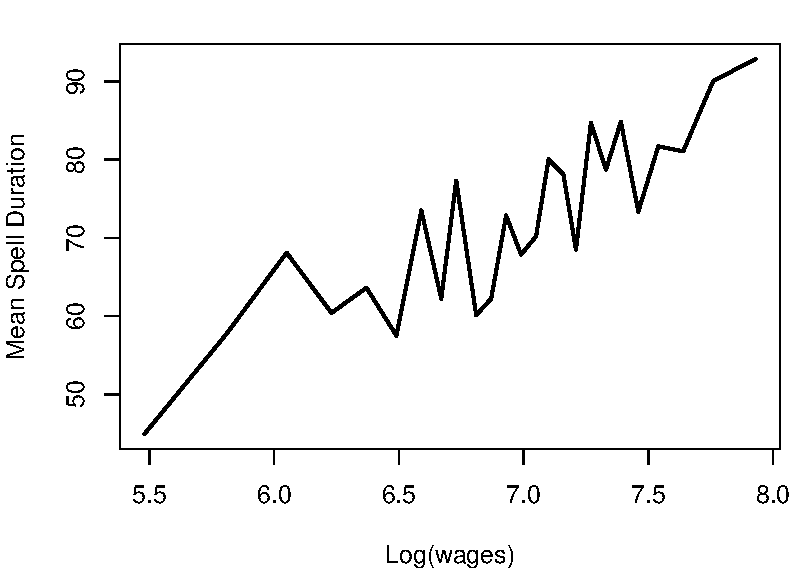
\includegraphics[scale=.6]{./pics/duration_wages.pdf}
    \caption{Variation in mean duration across wage percentiles}
    \label{fig:duration}
  \end{figure}

\item Explain how one can obtain a non-parametric estimate of the wage
  sampling distribution $F$ from the data. Construct this
  non-parametric estimate, and plot it on the same graph as
  \texttt{G}. Is this consistent with the theory? What else can you
  say about the estimate of $F$? \\ \Hline \\
  As mentioned in the slides, the cdf of wages accepted by workers who
  were just hired from unemployment provides a direct estimator
  $\hat F$ of the sampling distribution. I construct the empirical CDF
  of F using the wages of newly hired from unemployment. Figure
  \ref{fig:Fhat} shows the empirical CDF of F and G estimated
  non-parametrically using the data on log wages. The solid gray line
  shows the empirical distribution function of $\hat F$ and the solid
  black line shows the empirical distribution function of $\hat G$.
  This is consistent with the theory that we learnt in class. Figure
  \ref{fig:Fhat} shows that $\hat G$ first order stochastically
  dominates $\hat F$. This is expected given the selection of workers
  into better jobs.
  \begin{figure}[htbp!]
    \floatintro{The figure shows the empirical cdf of $F$ and $G$
      estimated from the data on wages using BHPS survey data. The
      solid gray line shows the empirical distribution function of
      $\hat F$ and the solid black line shows the empirical
      distribution function of $\hat G$.}  \centering
    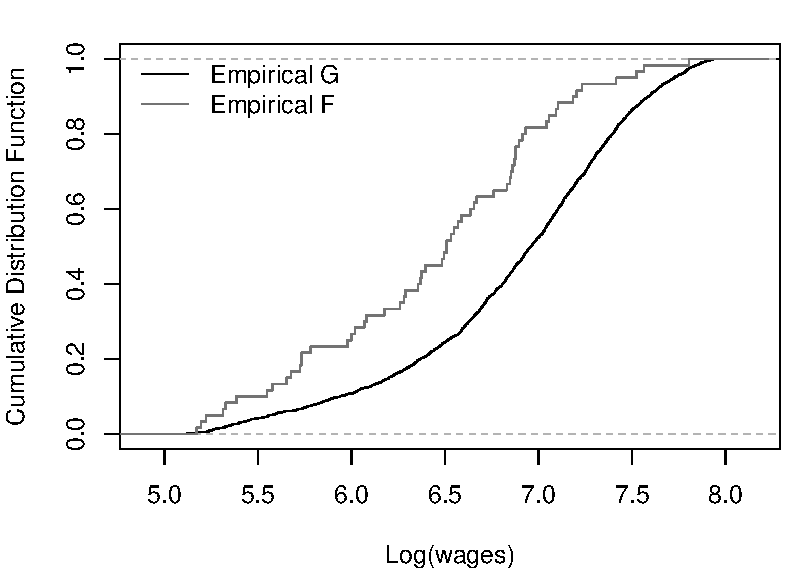
\includegraphics[scale=.6]{./pics/FG_data.pdf}
    \caption{Non-parametric estimate of empirical CDF ($\hat F$ and
      $\hat G$)}
    \label{fig:Fhat}
  \end{figure}
  \begin{figure}[htbp!]
    \floatintro{The figure shows the empirical pdf of $f$ and $g$
      estimated from the data on wages using BHPS survey data. The
      solid gray line shows the kernel density estimate of $\hat f$
      and the solid black line shows the kernel density estimate of
      $\hat g$.}  \centering
    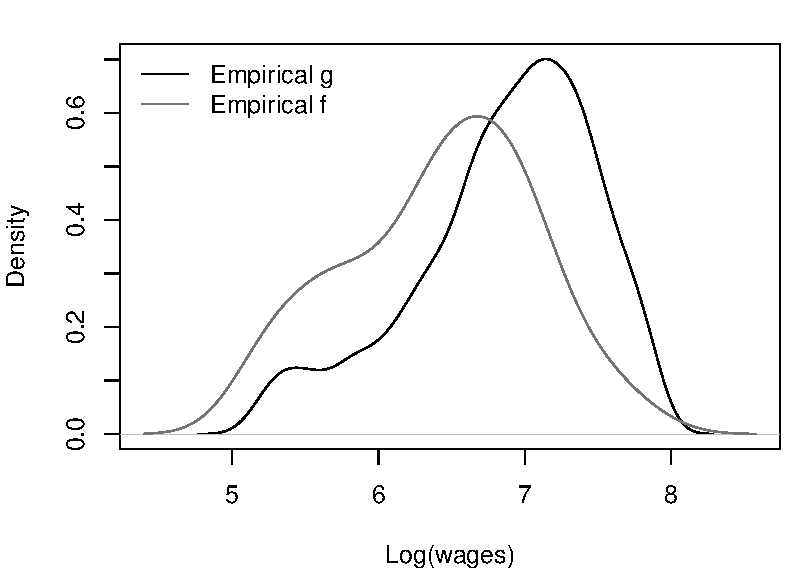
\includegraphics[scale=.6]{./pics/FG_density.pdf}
    \caption{Kernel density estimate of PDF ($\hat f$ and $\hat g$)}
    \label{fig:Gdens}
  \end{figure}
\end{enumerate}
\section{Estimation}
\begin{enumerate}
\item Write code for the MLE estimation of the BM model following the
  two-step protocol of Bontemps, Robin and Van den Berg (1999). \\
  \Hline \\
  I follow the two-step protocol as laid out in Bontemps, Robin and
  Van den Berg (2000)\footnote{I think the paper you wanted to refer
    to was the 2000 one and not the 1999 one. The lecture slides say
    that it is the 2000 one.}. Given our estimates of $\hat G$ and
  $\hat g$, I write functions $\hat F(:,\kappa_1)$ and
  $\hat f(:,\kappa_1)$ as functions of
  $\kappa_1 = \frac{\lambda_1}{\delta}$. These expressions are given
  as:
  \begin{align*}
    \hat F(w) = \frac{(1+\kappa_1) \hat G(w)}{1+\kappa_1 \hat G(w)}
    \qquad \text{and} \qquad
    \hat f(w) = \frac{(1+\kappa_1) \hat g(w)}{[1+\kappa_1 \hat G(w)]^2}
  \end{align*}

  Next, I write the likelihood function for the employed and
  unemployed using the expressions below:
  \begin{align*}
    L(x_i | e_1=0) &= \lambda_0^{1-c_i} exp(-\lambda_0 d_i)
                     f(y_{0i})^{1-c_i}\\
    L(x_i | e_i=1) &= g(y_{i1}) (\delta+ \lambda_1 \bar
                     F(y_{i1}))^{1-c_i} exp((-\delta+\lambda_1 \bar F(y_{i1}))d_i)
                     \bigg( \frac{\delta}{\delta + \lambda_1 \bar
                     F(y_{i1}}\bigg)^{\tau_{JUi}} \bigg(\frac{\lambda_1 \bar
                     F(y_{i1})}{\delta + \lambda_1 \bar F(y_{i1})}\bigg)^{\tau_{JJi}}
  \end{align*}
  The generic likelihood contribution of an observation $x_i$ is
  therefore:
  \begin{align*}
    L(x_i) = \bigg(\frac{\lambda_0}{\delta+\lambda_0}
    L(x_i|e_i=1)\bigg)^{e_i} \bigg(\frac{\delta}{\delta+\lambda_0} L(x_i|e_i=0)\bigg)^{1-e_i}
  \end{align*}
  which is a function of $F$, $G$ and the parameters $\delta$,
  $\lambda_0$, and $\lambda_1$ Finally, I take the natural logarithms
  of these, add them up and minimise the negative of the log
  likelihood using a routine optimisation in \texttt{R}.  The solver
  converges and the values for these parameters are given by:
  $\lambda_0=0.1496$, $\lambda_1=0.01359$, and $\delta=0.01$ which
  gives a value of $\kappa_1 = \frac{\lambda_1}{\delta}=1.3591$.
\item Write code for computing the standard errors of the estimates
  $\delta$, $\lambda_0$ and $\lambda_1$, explaining the assumptions
  upon which those standard errors rely. \\ \Hline \\
\item The file \texttt{BM\_data\_simulated.csv} contains artificial
  data resulting from a simulation of 5,000 workers behaving according
  to the BM model with parameters $\delta=0.01$, $\lambda_0=0.1$,
  $\lambda_1=0.05$ (monthly values). Run your ML estimation routine on
  the simulated data, and check that your estimates against the true
  parameter values. \\ \Hline \\
  Note that the simulated data does not have a column for wages of
  unemployed who were hired. But, from the lecture slides, one can see
  that if wage is unobserved, we can integrate out the wages from the
  likelihood expression and re-write it as:

  I use this fact and then run the ML estimation routine as before on
  the simulated data set. My parameter estimates are
  $\lambda_0=0.09986$, $\lambda_1=0.05385$ and $\delta=0.00999$. These
  are close to the true parameter values. Therefore, it gives us a
  sanity check as to if the ML estimation routine works well enough or
  not.
\end{enumerate}
\section{Playing around with the model}
\begin{enumerate}
\item What is the predicted unemployment rate from the estimates
  obtained in Section II? Compare it with the sample unemployment
  rate, and discuss the possible reasons for any discrepancy. \\
  \Hline \\
  Given our estimates of the parameters and the steady state
  assumption, the sample unemployment rate can be calculated as:
  \begin{align*}
    Pr\{e_i=0\} = 1-Pr\{e_i=1\} = \text{Unemp. rate} =
    \frac{\delta}{\delta+\lambda_0}
  \end{align*}
For BHPS data, the sample unemployment rate is 5.92\% whereas the
predicted unemployment rate from the MLE estimation of parameters is
6.26\%. For simulated data, the sample unemployment rate is 9.58\% whereas
the predicted unemployment rate from the MLE estimation is 9.09\%.
\item Construct kernel density estimates of the cross-section
  distribution of wages $g(w)$ and of the sampling distribution
  $f(w)$. Plot both densities on the same graph. \\ \Hline \\
Figure \ref{fig:Gdens} shows the kernel density estimates for the BHPS
data. These kernel density estimates are from the sample itself and
not from the predictions of our estimation routine. 
\item Construct the distribution of firm productivity that
  rationalises the observed wage distribution within the BM
  model. Plot firm productivity against wages, and against the
  cross-section CDF of wages $G(w)$. Do you notice anything wrong? \\ \Hline \\
\item Looking at the predicted profit rate of high-productivity firms,
  what else can you say about the BM model? \\ \Hline \\
\end{enumerate}
\newpage
\begin{appendix}
\section{Mean duration across wage percentiles}
\begin{table}[htbp!]
  \centering
  \input{./tables/duration_wages_float.gen}
  \caption{Variation in mean duration across wage percentiles}
  \label{tab:duration}
\end{table}
\end{appendix}
\end{document}
